\chapter{KẾT LUẬN VÀ HƯỚNG PHÁT TRIỂN}

\section{Kết luận}

Nhận dạng ngôn ngữ ký hiệu hay dịch ngôn ngữ ký hiệu cho người khiếm thính là một trong những đề tài mang tính nhân văn cao, giúp đỡ người khiếm thính hòa nhâp cộng đồng. Qua các phần nội dung chính, luận văn đã tìm hiểu cũng như áp dụng các thuật toán đi từ đầu đến cuối quá trình hoạt động của ứng dụng nhận dạng ngôn ngữ ký hiệu. Ban đầu từ camera RGB, ảnh được xử lý quá mạng ước tính tư thế khung xương để xác định các vector đặc trưng khung xương của từng người (SJM). Sau đó các SJM được xử lý qua các bước loại bỏ khớp xương không cần thiết, chuẩn hóa tọa độ khớp xương. Tiếp sau đó các SJM sau xử lý được đưa qua mạng NN để phân loại ra tư thế đó thuộc lớp nào. Cuối cùng sử dụng giải thuật Deep Sort để theo dõi từng từ ngữ diễn đạt của mỗi người. Ứng dụng tương tác với người sử dụng qua giao diện được viết bằng thư viện PyQt5.
\newpage
Từ mục tiêu ban đầu đề ra, tuy gặp phải khó khăn nhưng qua quá trình tìm tòi và được sự hướng dẫn của thầy Hà Hoàng Kha, luận văn đã hoàn thành được những mục tiêu:
\begin{itemize}
\item Luận văn đã trình bày cơ bản lý thuyết về các thuật toán trong machine learning và deep learning được sử dụng hiện nay. Tìm hiểu về các phương pháp được sử dụng trong việc nhận dạng ngôn ngữ ký hiệu. Trong số đó phương pháp sử dụng mạng NN để ước tính tư thế khung xương.
\item Luận văn đã áp dụng mô hình ước lượng tư thế khung xương để đưa vào ứng dụng. Mô hình ước lượng được tọa độ 18 khớp xương chính trên cơ thể và có khả năng dự đoán đối với nhiều người trong khung hình cùng một lúc.

\item Xây dựng được mô hình nhận dạng ngôn ngữ ký hiệu từ các SJM được xuất ra từ mô hình ước lượng tư thế khung xương. Mô hình phân loại được 16 lớp ứng với 16 từ ngữ trong bộ từ ngữ ngôn ngữ ký hiệu. Mô hình đạt được tỷ lệ nhận dạng cao trong điều kiện thực tế.

\item Áp dụng giaỉ thuật Deep Sort để theo dõi từng người và từ ngữ họ diễn đạt.

\item Sau cùng luận văn đã xây dựng thành công ứng dụng nhận dạng ngôn ngữ ký hiệu và theo dõi cho người khiếm thính. Với giao diện thân thiện với người dùng. ứng dụng có khả khả năng xử lý realtime từ việc ước tính tư thế, dự đoán từ ngữ cho đến theo dõi đối với nhiều người cùng lúc. Ứng dụng có tốc độ xử lý ổn định trên các thiết bị cấu hình thấp.
\end{itemize}

Tuy nhiên luận văn vẫn còn rất nhiều những nhược điểm chưa giải quyết được :
	\begin{itemize}
	\item Ngôn ngữ ký hiệu Việt Nam đặc trưng là sự kết hợp của cả tư thế con người với cử động của cánh tay, bàn tay và sắc thái khuôn mặt. Tuy nhiên, mạng ước tính tư thế khung xương được luận văn sử dụng chỉ mới ước tính được cơ bản tư thế con người với 18 khớp xương được xác định trong không gian 2D. Việc này khiến cho nó có những nhược điểm: 
\begin{itemize}
	\item Mô hình vẫn chưa ước lượng được đến hình dáng bàn tay, các ngón tay và nét mặt. Do vậy mạng NN chưa thể học được các thủ ngữ dựa trên chuyển động của các ngón tay và nét mặt.
	\item Mô hình mới chỉ ước tính tư thế trên không gian 2D. Do vậy khi thay đổi hướng quan sát của camera, sang hướng khác không phải trực diện thì ứng dụng sẽ không nhận dạng chính xác được.
	\item Mô hình nhận dạng thủ ngữ mới chỉ dự đoán được trên từng SJM riêng biệt. Do vậy mô hình mới chỉ dự đoán được đối với những từ ngữ mà tư thế không thay đổi nhiều hoặc chuyển động ít. Đối với những từ ngữ cần phải kết hợp nhiều tư thế, mạng vẫn chưa xử lý được.
	\end{itemize}
\item Số lượng từ ngữ mà mô hình nhận dạng được mới chỉ dừng lại ở 16 từ ngữ ký hiệu. Trong khi đó số lượng từ ngữ trong ngôn ngữ ký hiệu Việt Nam lên đến hàng trăm nghìn. Do vậy vẫn chưa thể đưa được ứng dụng vào thực tế.

\item Ứng dụng mới chỉ được xây dựng trên máy tính trong khi đó yêu cầu đặt ra là đưa ứng dụng lên điện thoại thông mình để hỗ trợ người dùng sử dụng ở mọi nơi.
\end{itemize}
\section{Hướng phát triển}
Với những nhược điểm còn tồn tại, để có thể đưa ứng dụng vào đời sống giúp đỡ người khiếm thính, cần phải giải quyết chúng một cách toàn diện và hiệu quả. Luận văn xin đề ra một số hướng để tiếp tục phát triển đề tài hoàn thiện tốt hơn:
\begin{itemize}
\item Xây dựng mô hình ước lượng tư thế tốt hơn. Để phát triển, ban đầu cần xây dựng mô hình ước tính cả tư thế và hình dáng bàn tay trong không gian 3D, ngoài ra có thể dự đoán thêm nét mặt. Một mô hình như vậy mới đủ để trích được các đặc trưng của một từ ngữ ký hiệu. 

\FloatBarrier
\begin{figure}[htp]
\begin{center}
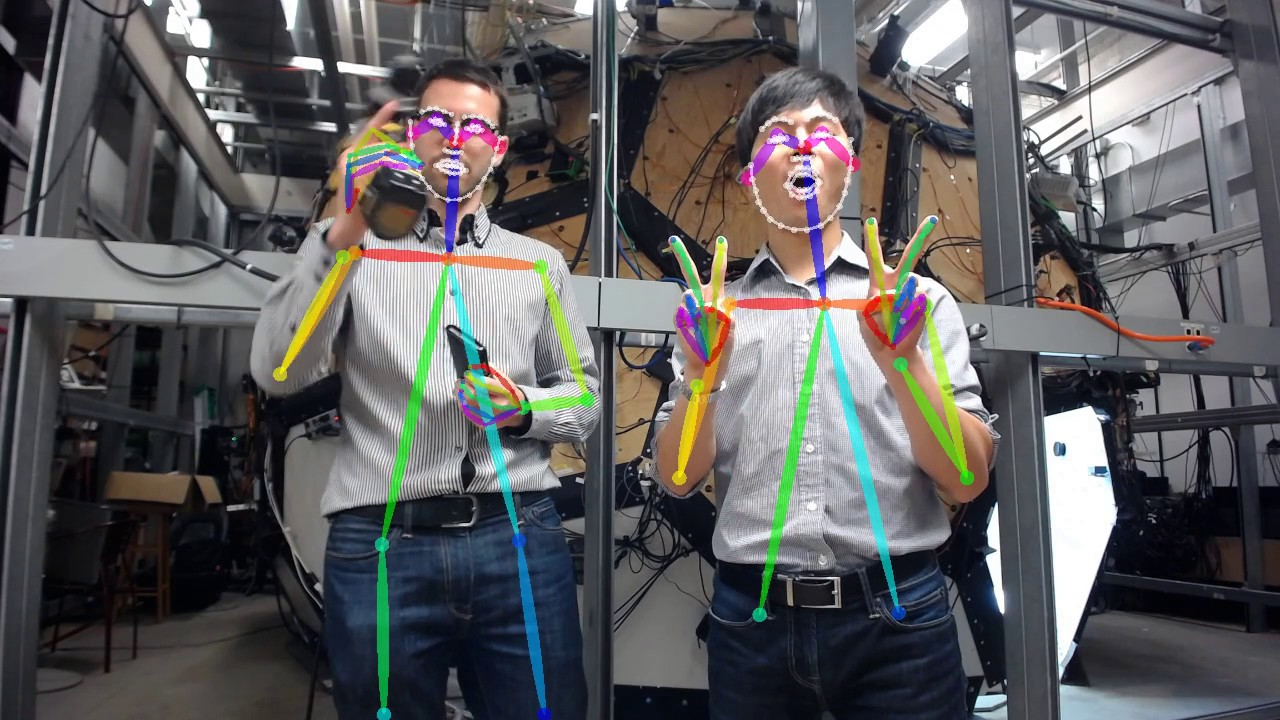
\includegraphics[scale=0.3]{chap7/c7_figs/open_pose.jpg}
\end{center}
\caption{Mô hình ước tính tư thế mà luận văn hướng tới \\ nguồn: thư viện openpose}
\label{fig:openpose}
\end{figure}
\FloatBarrier

\item Xây dựng mô hình nhận dạng từ ngữ dựa trên các chuỗi SJM theo thời gian thay vì dự đoán dựa trên các SJM riêng biệt. Việc này cần sự ứng dụng của các mô hình như LSTM hoặc CNN-LSTM để dự đoán được.

\item Nâng cấp mô hình để có thể dự đoán được nhiều từ ngữ hơn mới có thể đưa ra ứng dụng thực tế.

\item Cần xây dựng ứng dụng có thể hoạt động trên điện thoại thông minh, giúp người dùng có thể sử dụng dễ dàng.

\end{itemize}
